\subsection{Muon Fake Rate}
This section presents in more detail the studies on the muon fake rate.

\subsubsection{Fakeable Object}
The muon fakeable object definition is simply the muon selection requirements (Sec.~\ref{sec:sel_muons}) 
but with looser $d_0$ and isolation thresholds. We study two definitions:
\begin{itemize}
  \item M1
  \begin{itemize}
    \item $|d_{0}| < 0.2$~cm
    \item $\frac{\rm{Iso}_{Total}}{\pt}~<~1.0$
  \end{itemize}
  \item M2 
  \begin{itemize}
    \item $|d_{0}| < 0.2$~cm
    \item $\frac{\rm{Iso}_{Total}}{\pt}~<~0.4$
  \end{itemize}
\end{itemize}
Note that M1 is the definition studied in~\cite{fakeLeptonNote2}. The motivation for the tighter selection 
of M2 is the reduction of systematic uncertainties by reducing the extrapolation in isolation.

\subsubsection{Calibration Sample Selection}
The muon fake rate has been measured in $5\ipb$ of data in Run2011A. The selected events are triggered
by any one of HLT\_Mu8 or HLT\_Mu15 single muon trigger paths. Addition requirements are also needed to
reduce contamination of the calibration sample with muons from $W$ and $Z$ decays and to tune the
jet composition:
\begin{itemize}
  \item $Z$ veto: reject the event if there are two oppositely charged muons satisfying the loose muon 
        selection and with $p_T>20\:\GeVc$,
  \item $W$ veto: reject the event if PF-MET $> 20\:\GeV$ or if the transverse mass of the loose muon 
        and PF-MET is above $20\:\GeVcc$,
  \item require the presence of a PF-jet with $p_T > 15\:\GeVc$ and separated by $\Delta R > 1$ 
        from the loose muon.
\end{itemize}
The jet threshold of $p_T > 15\:\GeVc$ (uncorrected) was found to best model the jet spectrum of the $W+$jets 
process according to~\cite{fakeLeptonNote2}. The jets used in this study has the L1FastJet, L2Relative, and
L3Absolute jet energy corrections applied. The issue of the jet threshold needs to be reviewed in the 2011 
data and Spring11 Monte Carlo samples.

\subsubsection{Fake Rates}
The fake rate parametrized in $\eta$-$p_T$ is listed in Tabs.~\ref{tab:mu_fr_iso1_jet15} and~\ref{tab:mu_fr_iso04_jet15}. 
Figs.~\ref{fig:mu_fr_iso1_jet15} and~\ref{fig:mu_fr_iso04_jet15} show how the fake rates trends when projected onto $p_T$ or $\eta$.

\begin{table}[!htbp]
\begin{center}
\begin{tabular}{|c|c|c|c|c|c|}
\hline
  & $0<\eta<0.5$ & $0.5<\eta<1$ & $1<\eta<1.5$ & $1.5<\eta<2$ & $2<\eta<2.4$ \\
\hline
$10 < p_T < 15$ & $0.0856 \pm 0.0044$ & $0.1016 \pm 0.0048$ & $0.1128 \pm 0.0050$ & $0.1265 \pm 0.0057$ & $0.1376 \pm 0.0096$ \\
\hline
$15 < p_T < 20$ & $0.0687 \pm 0.0019$ & $0.0768 \pm 0.0021$ & $0.0897 \pm 0.0024$ & $0.1078 \pm 0.0029$ & $0.1060 \pm 0.0054$ \\
\hline
$20 < p_T < 25$ & $0.0991 \pm 0.0046$ & $0.1231 \pm 0.0052$ & $0.1467 \pm 0.0059$ & $0.1608 \pm 0.0068$ & $0.1901 \pm 0.0136$ \\
\hline
$25 < p_T < 30$ & $0.1056 \pm 0.0086$ & $0.1194 \pm 0.0092$ & $0.1189 \pm 0.0102$ & $0.1764 \pm 0.0136$ & $0.1769 \pm 0.0251$ \\
\hline
$30 < p_T < 35$ & $0.0804 \pm 0.0130$ & $0.0958 \pm 0.0147$ & $0.1407 \pm 0.0195$ & $0.1852 \pm 0.0241$ & $0.2637 \pm 0.0543$ \\
\hline
$35 < p_T < 40$ & $0.1429 \pm 0.0268$ & $0.1043 \pm 0.0255$ & $0.1719 \pm 0.0292$ & $0.1473 \pm 0.0381$ & $0.1957 \pm 0.0764$ \\
\hline
\end{tabular}
\caption{Muon fake rate in $\eta$-$p_T$ for M1 definition. Uncertainties are statistical only.}
\label{tab:mu_fr_iso1_jet15}
\end{center}
\end{table}

\begin{table}[!htbp]
\begin{center}
\begin{tabular}{|c|c|c|c|c|c|}
\hline
  & $0<\eta<0.5$ & $0.5<\eta<1$ & $1<\eta<1.5$ & $1.5<\eta<2$ & $2<\eta<2.4$ \\
\hline 
$10 < p_T < 15$ & $0.1813 \pm 0.0088$ & $0.2034 \pm 0.0090$ & $0.2154 \pm 0.0089$ & $0.2258 \pm 0.0096$ & $0.2557 \pm 0.0164$ \\
\hline
$15 < p_T < 20$ & $0.1548 \pm 0.0041$ & $0.1682 \pm 0.0043$ & $0.1829 \pm 0.0046$ & $0.2009 \pm 0.0051$ & $0.1942 \pm 0.0093$ \\
\hline
$20 < p_T < 25$ & $0.2489 \pm 0.0105$ & $0.2903 \pm 0.0109$ & $0.2996 \pm 0.0108$ & $0.3190 \pm 0.0122$ & $0.3501 \pm 0.0222$ \\
\hline
$25 < p_T < 30$ & $0.2641 \pm 0.0195$ & $0.3116 \pm 0.0210$ & $0.2692 \pm 0.0209$ & $0.3376 \pm 0.0231$ & $0.3291 \pm 0.0416$ \\
\hline
$30 < p_T < 35$ & $0.2130 \pm 0.0316$ & $0.2392 \pm 0.0332$ & $0.3240 \pm 0.0387$ & $0.3429 \pm 0.0396$ & $0.4800 \pm 0.0802$ \\
\hline
$35 < p_T < 40$ & $0.3434 \pm 0.0542$ & $0.3194 \pm 0.0642$ & $0.3551 \pm 0.0522$ & $0.2969 \pm 0.0680$ & $0.3750 \pm 0.1229$ \\
\hline
\end{tabular}
\caption{Muon fake rate in $\eta$-$p_T$ fro M2 definition. Uncertainties are statistical only.}
\label{tab:mu_fr_iso04_jet15}
\end{center}
\end{table}

\begin{figure}[!htbp]
\begin{center}
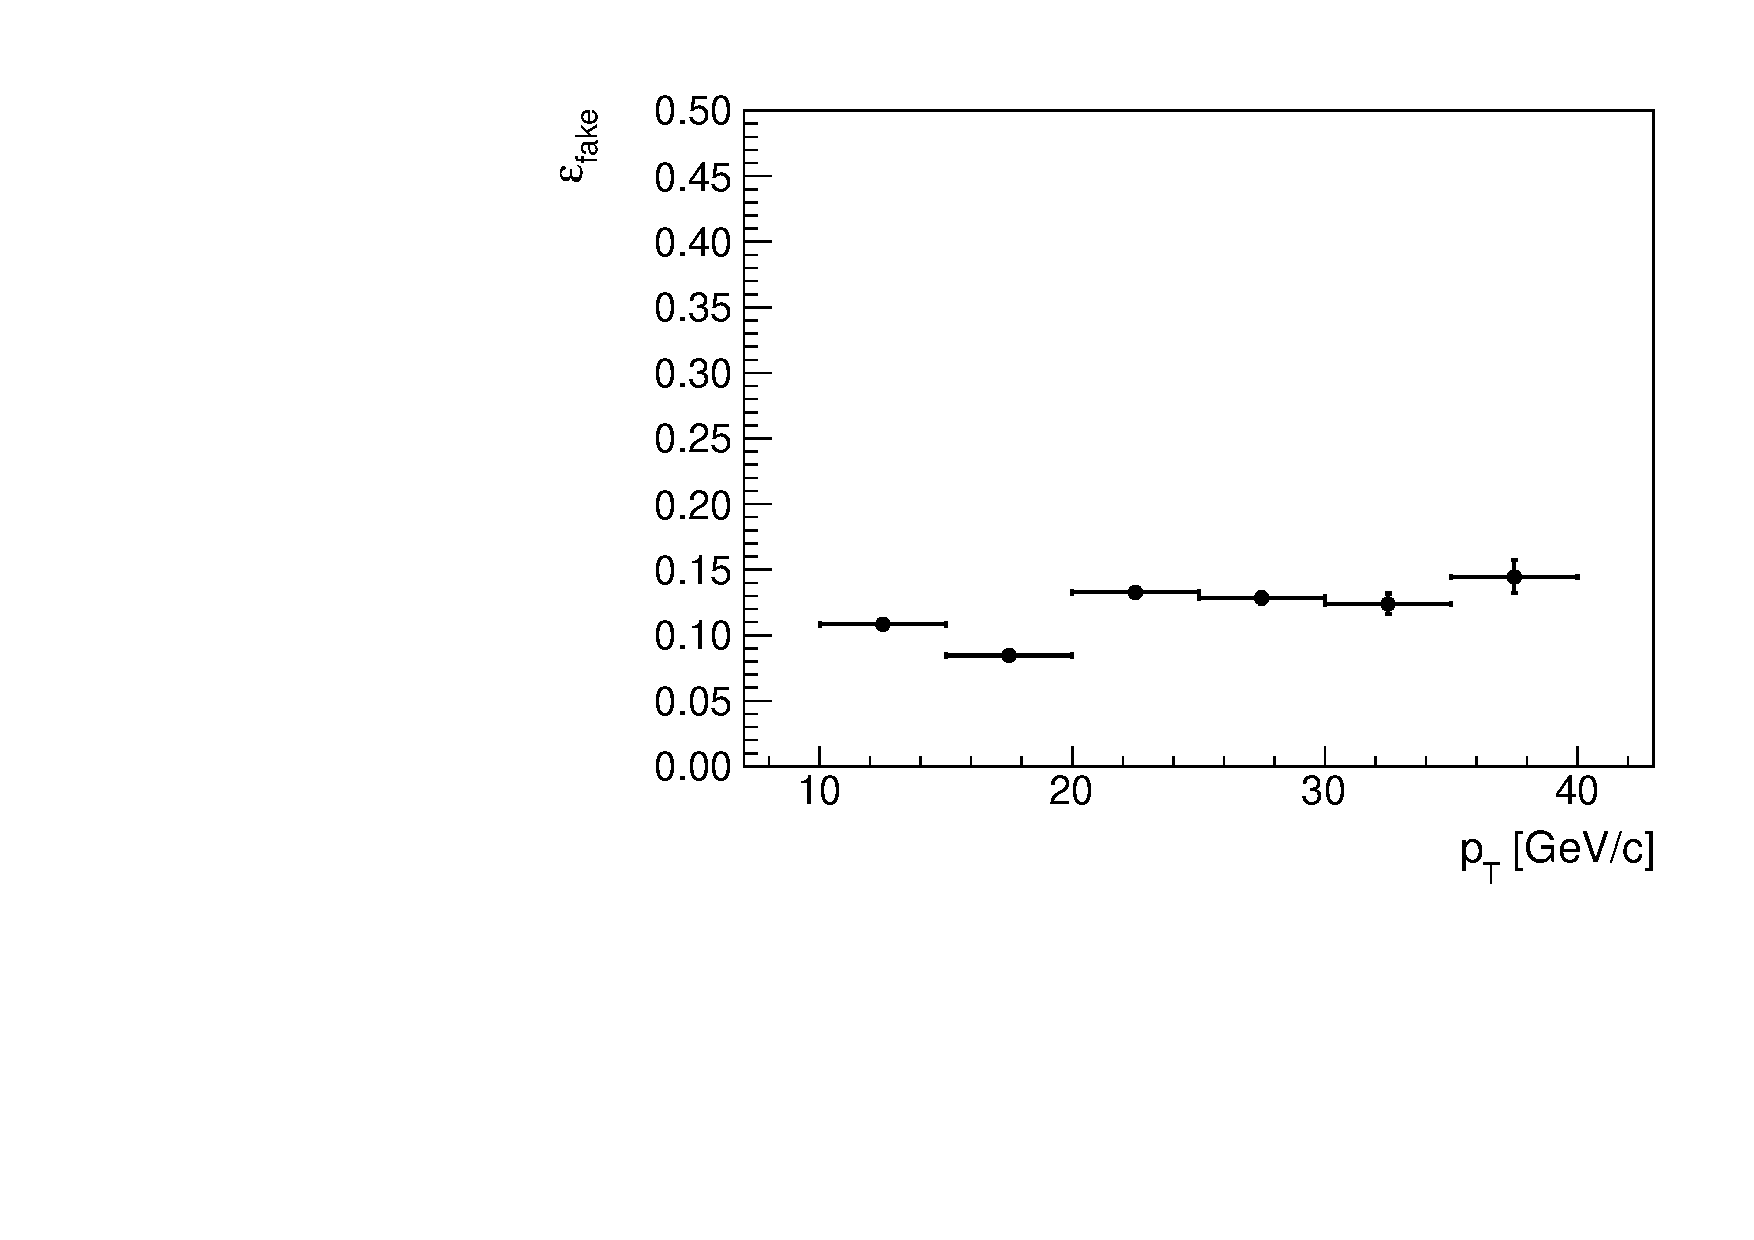
\includegraphics[width=0.45\textwidth]{figures/muon_frpt_m1.pdf}
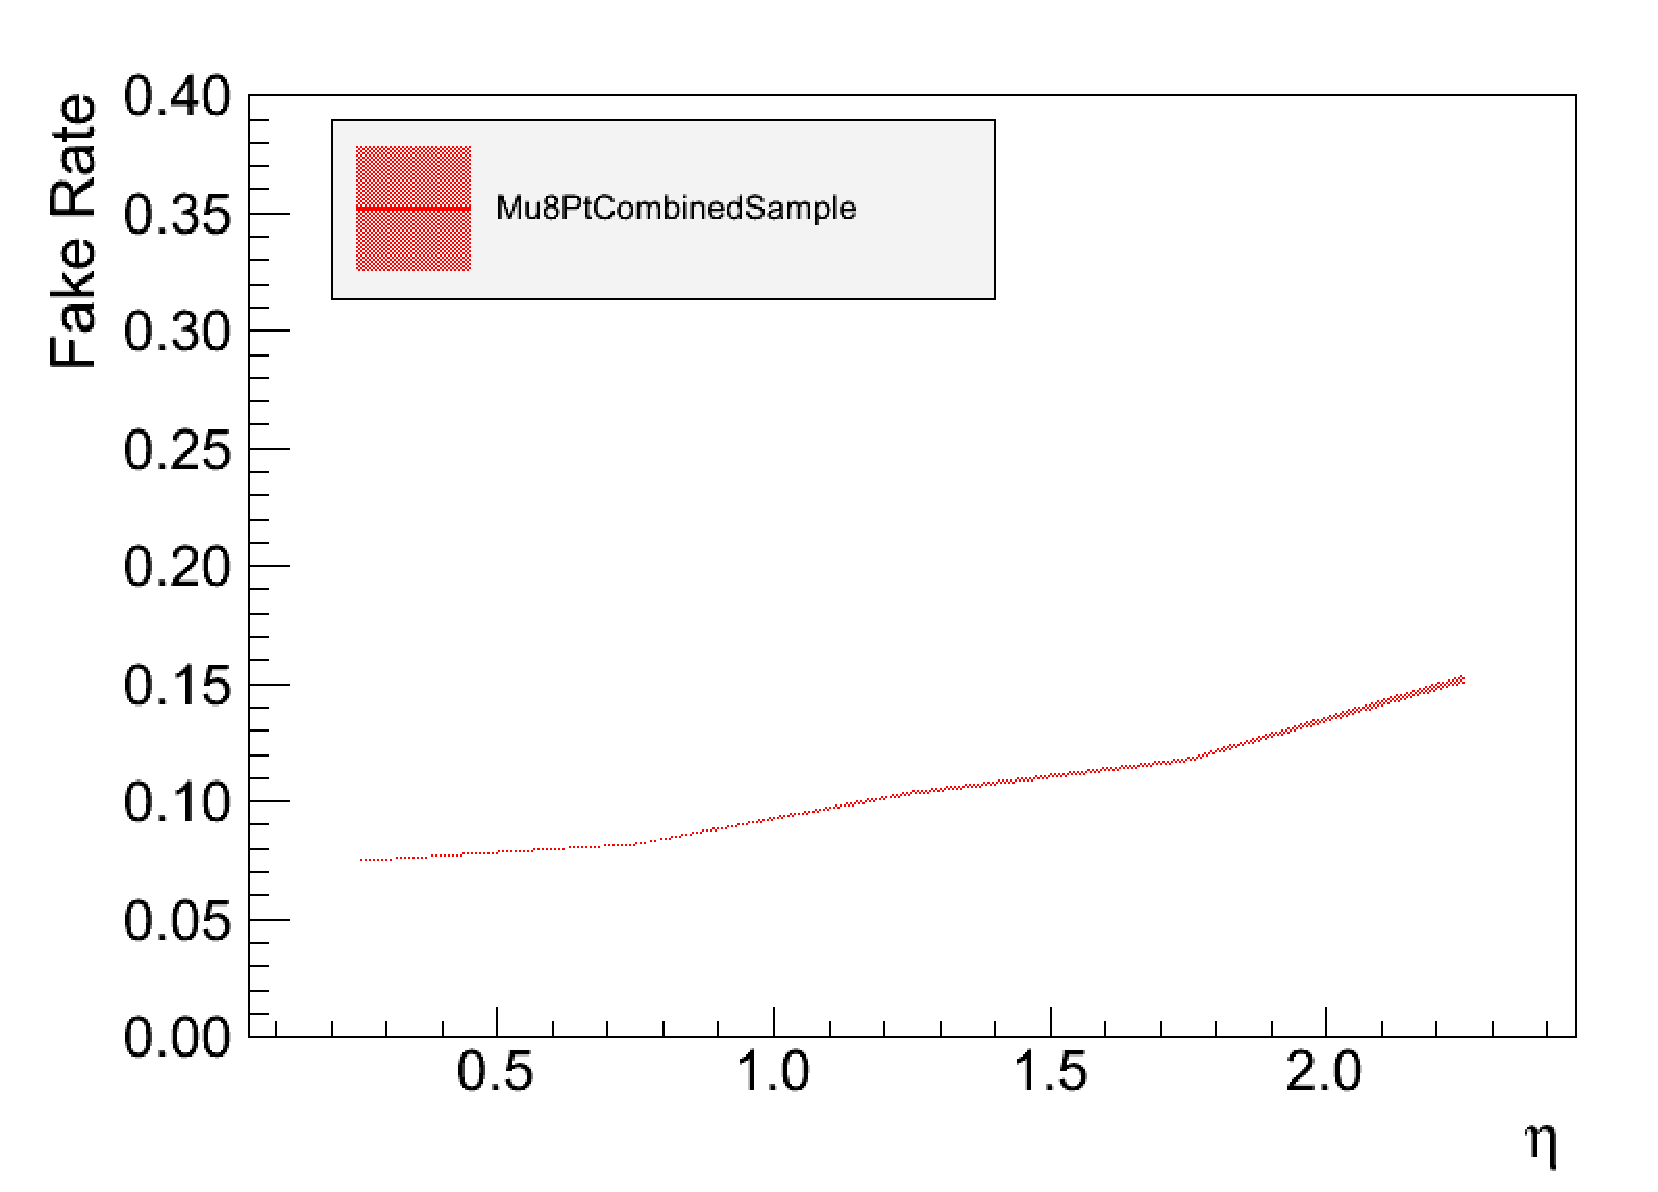
\includegraphics[width=0.45\textwidth]{figures/muon_freta_m1.pdf}
\caption{Fake rates for M1 definition projected onto $p_T$ and $\eta$.}
\label{fig:mu_fr_iso1_jet15}
\end{center}
\end{figure}

\begin{figure}[!htbp]
\begin{center}
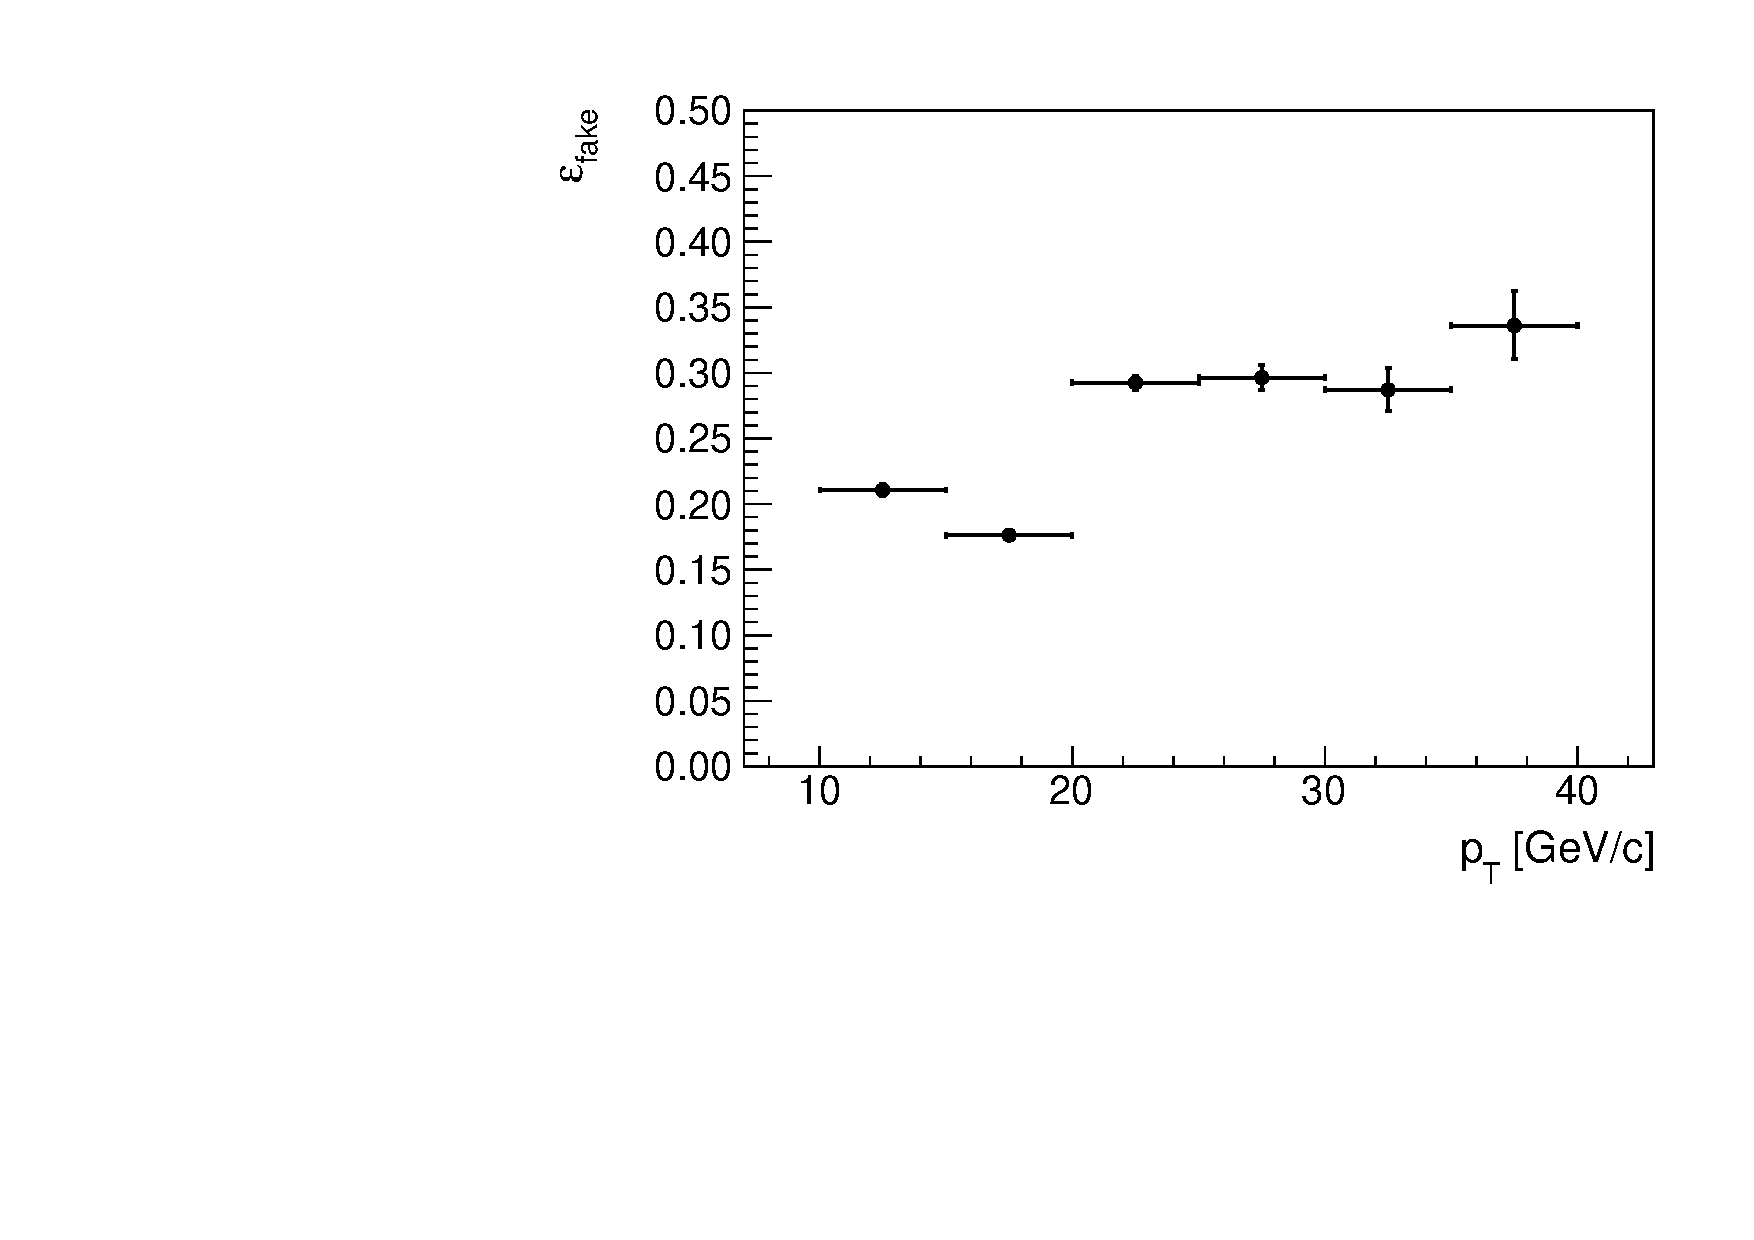
\includegraphics[width=0.45\textwidth]{figures/muon_frpt_m2.pdf}
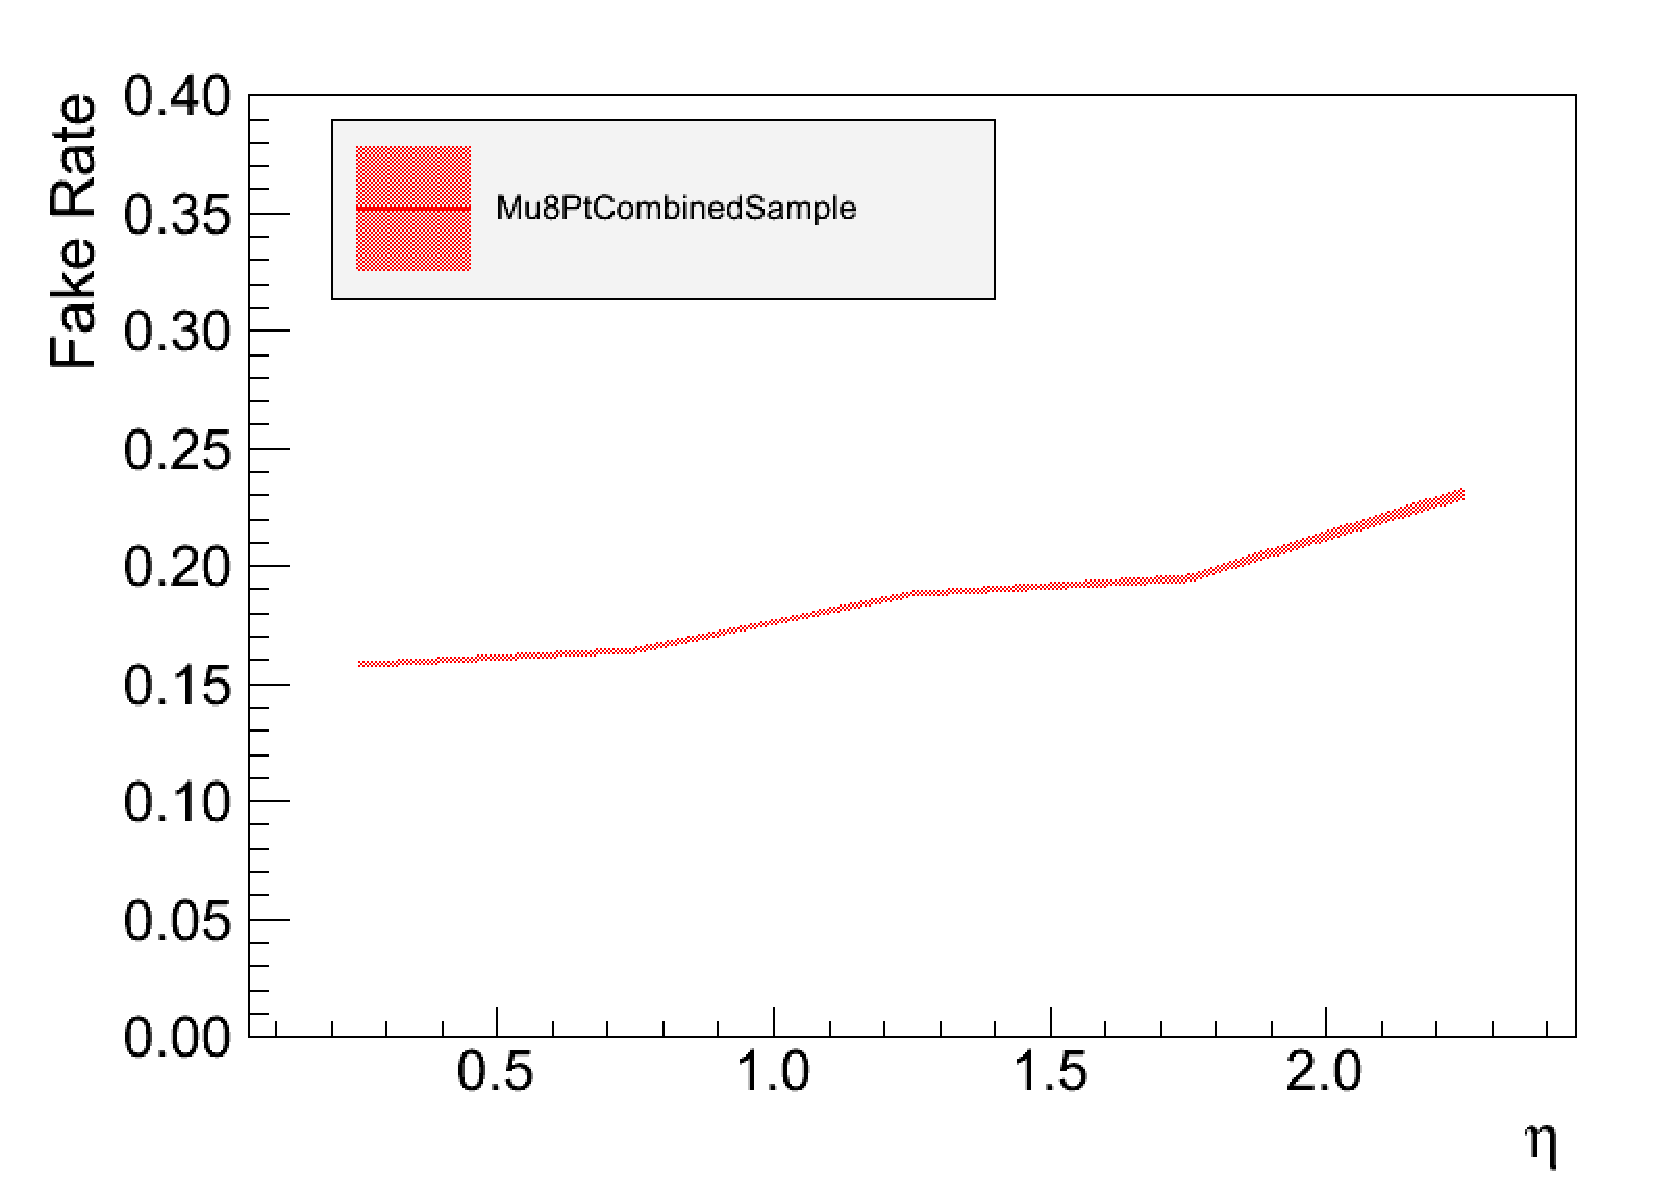
\includegraphics[width=0.45\textwidth]{figures/muon_freta_m2.pdf}
\caption{Fake rates for M2 definition projected onto $p_T$ and $\eta$.}
\label{fig:mu_fr_iso04_jet15}
\end{center}
\end{figure}

\subsubsection{Sample Dependence}
The systematic uncertainty associated with the jet sample dependence is estimated by measuring the difference in the
fake rate when the jet threshold is changed. In addition to the standard calibration sample defined previously, we
also measure the fake rate in a sample defined by a jet $p_T>30\:\GeVc$ threshold and in a sample without a jet
requirement. The largest difference from the nominal fake rate is taken as the systematic uncertainty. The 
systematic uncertainties are summarized in Tab.~\ref{tab:mu_fr_samp_dep}. The fake rate
projections onto $p_T$ and $\eta$ for various jet requirements are shown in Fig.~\ref{fig:mu_fr_iso04}. 

\begin{table}[!htbp]
\begin{center}
\begin{tabular}{|c|cc|c|}
\hline
FO & $p_T<20$ & $p_T>20$ & Overall \\
\hline 
M1 & $46\%$ & $29\%$ & $36\%$ \\
M2 & $29\%$ & $16\%$ & $19\%$ \\
\hline
\end{tabular}
\caption{Systematic uncertainties from sample dependence.}
\label{tab:mu_fr_samp_dep}
\end{center}
\end{table}

\begin{figure}[!htbp]
\begin{center}
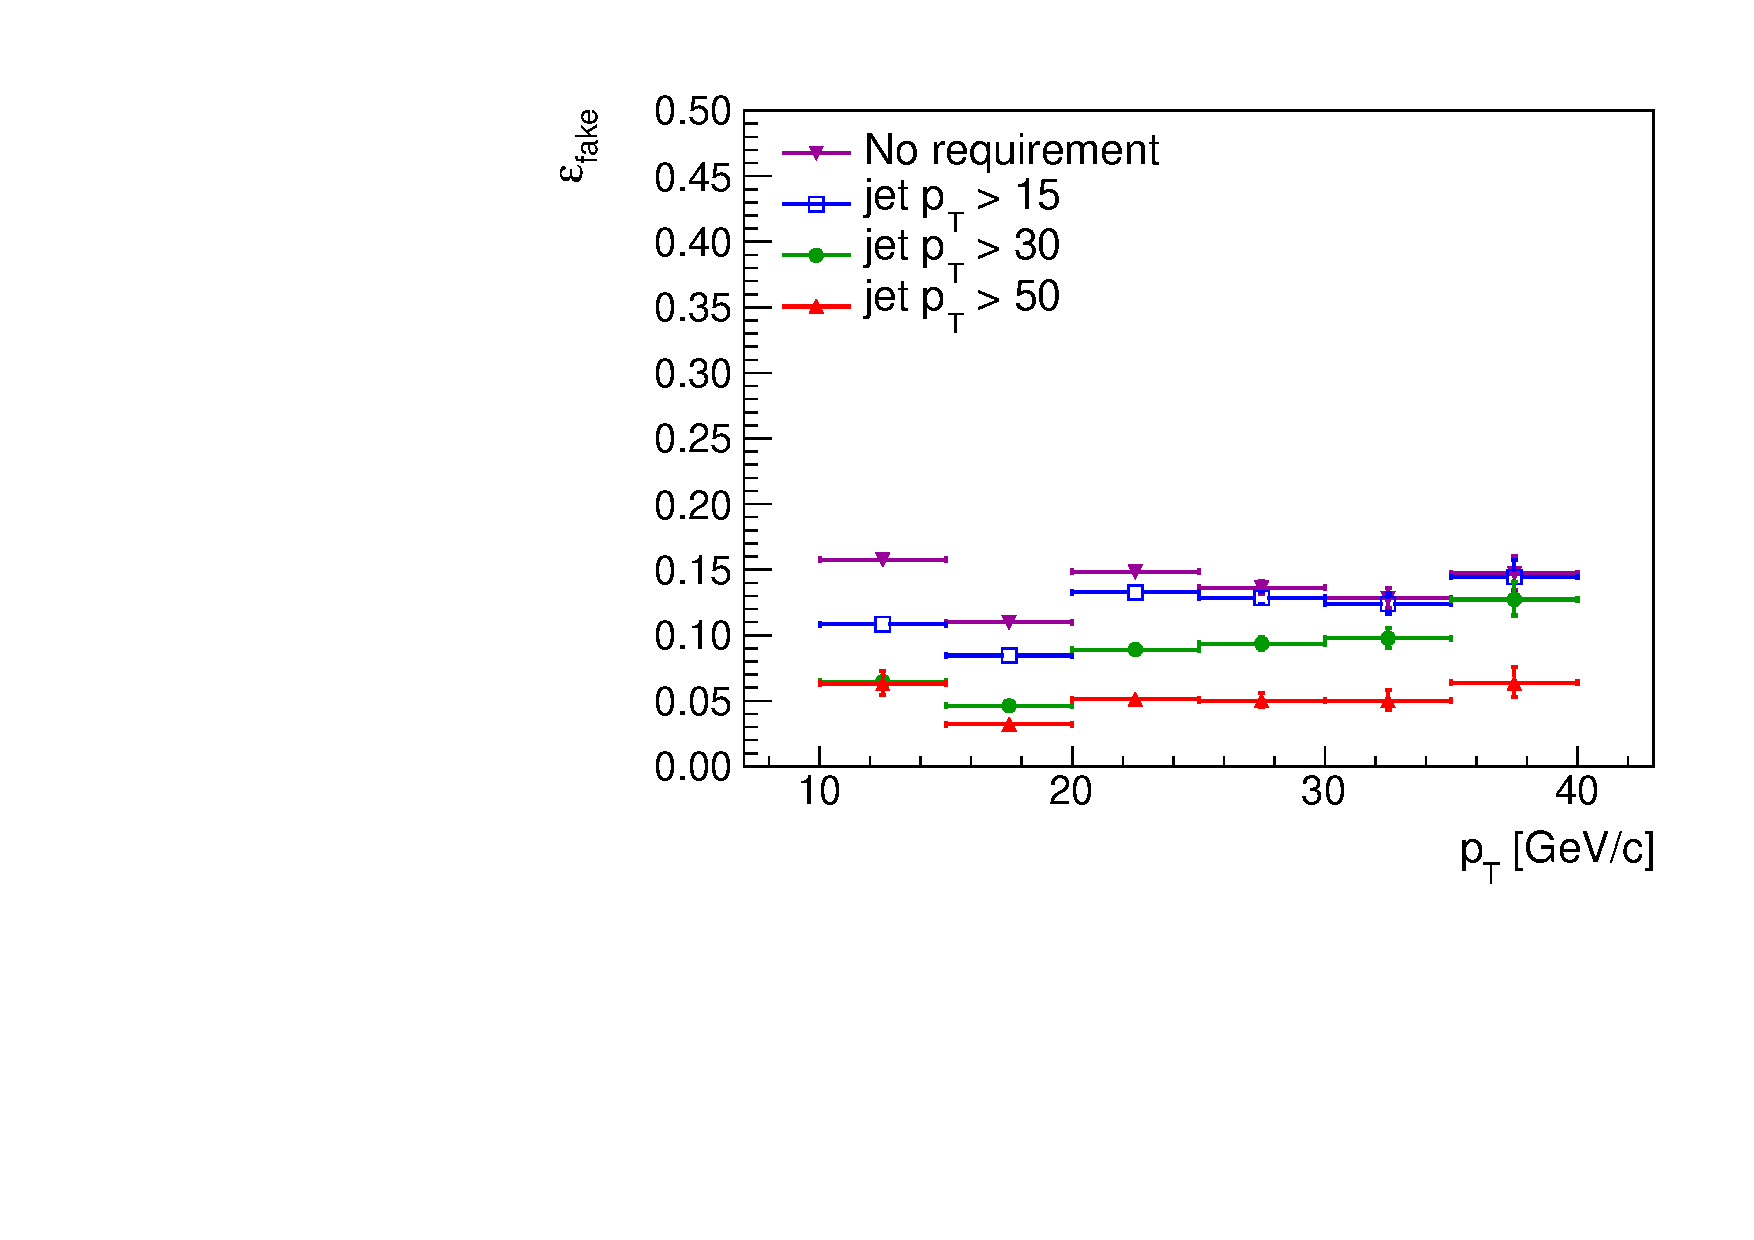
\includegraphics[width=0.45\textwidth]{figures/muon_frpt_jetscan_m1.pdf}
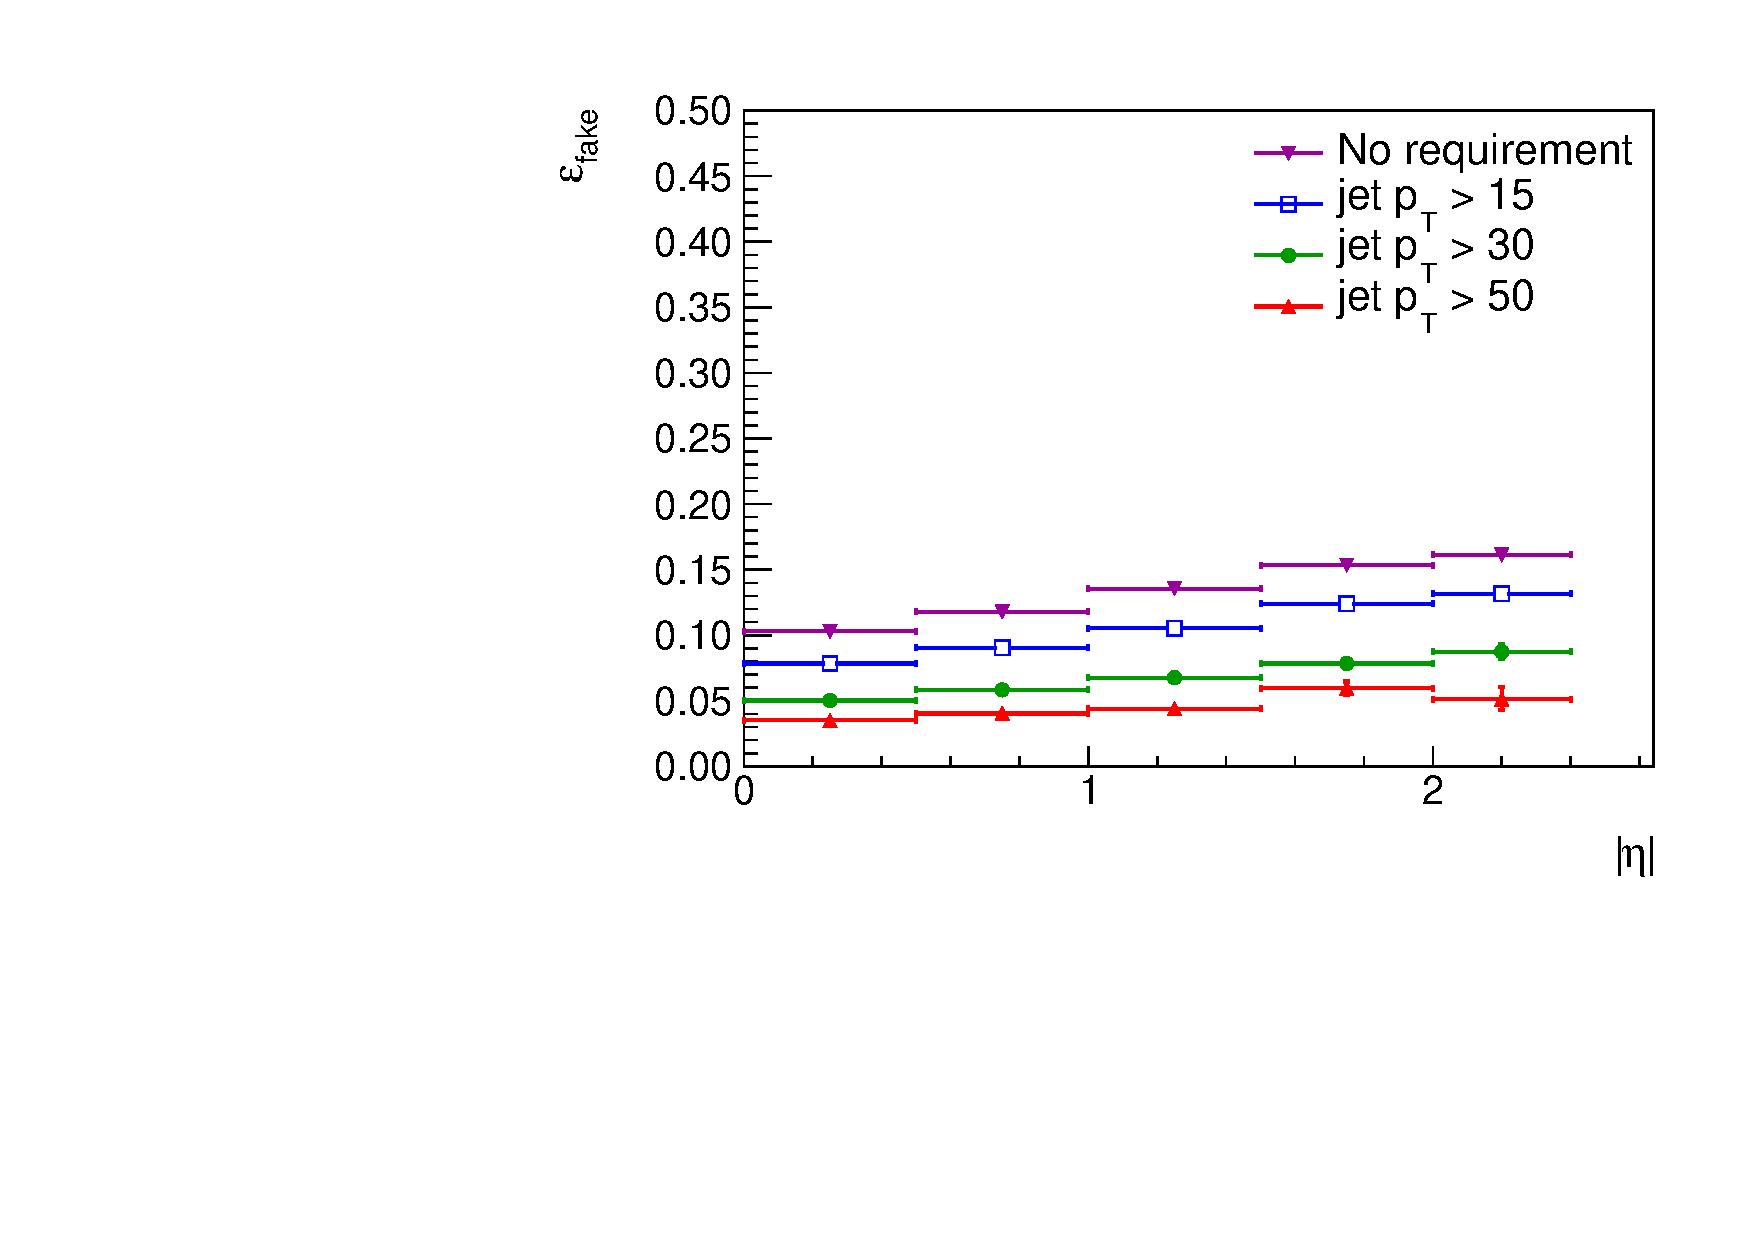
\includegraphics[width=0.45\textwidth]{figures/muon_freta_jetscan_m1.pdf}
\caption{Fake rates for M1 projected onto $p_T$ and $\eta$.}
\label{fig:mu_fr_iso1}
\end{center}
\end{figure}

\begin{figure}[!htbp]
\begin{center}
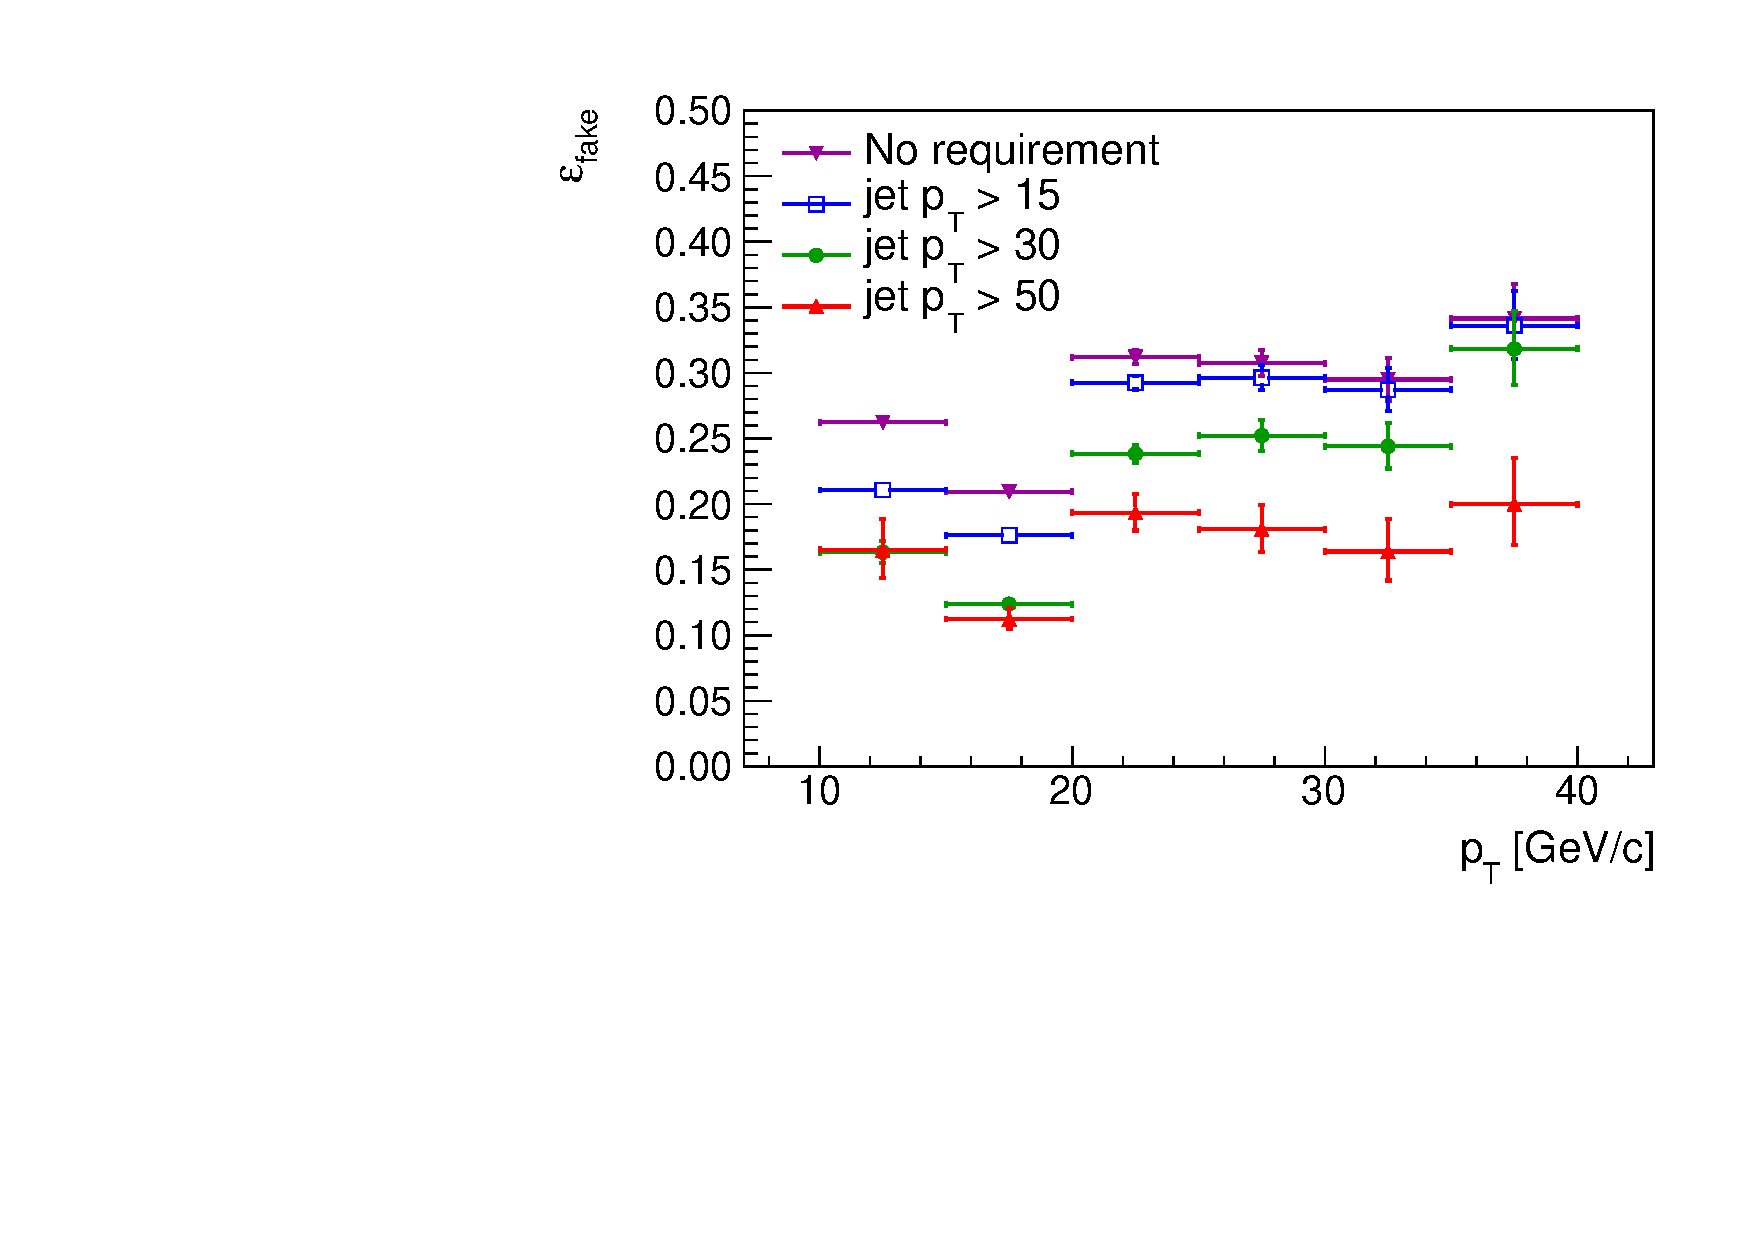
\includegraphics[width=0.45\textwidth]{figures/muon_frpt_jetscan_m2.pdf}
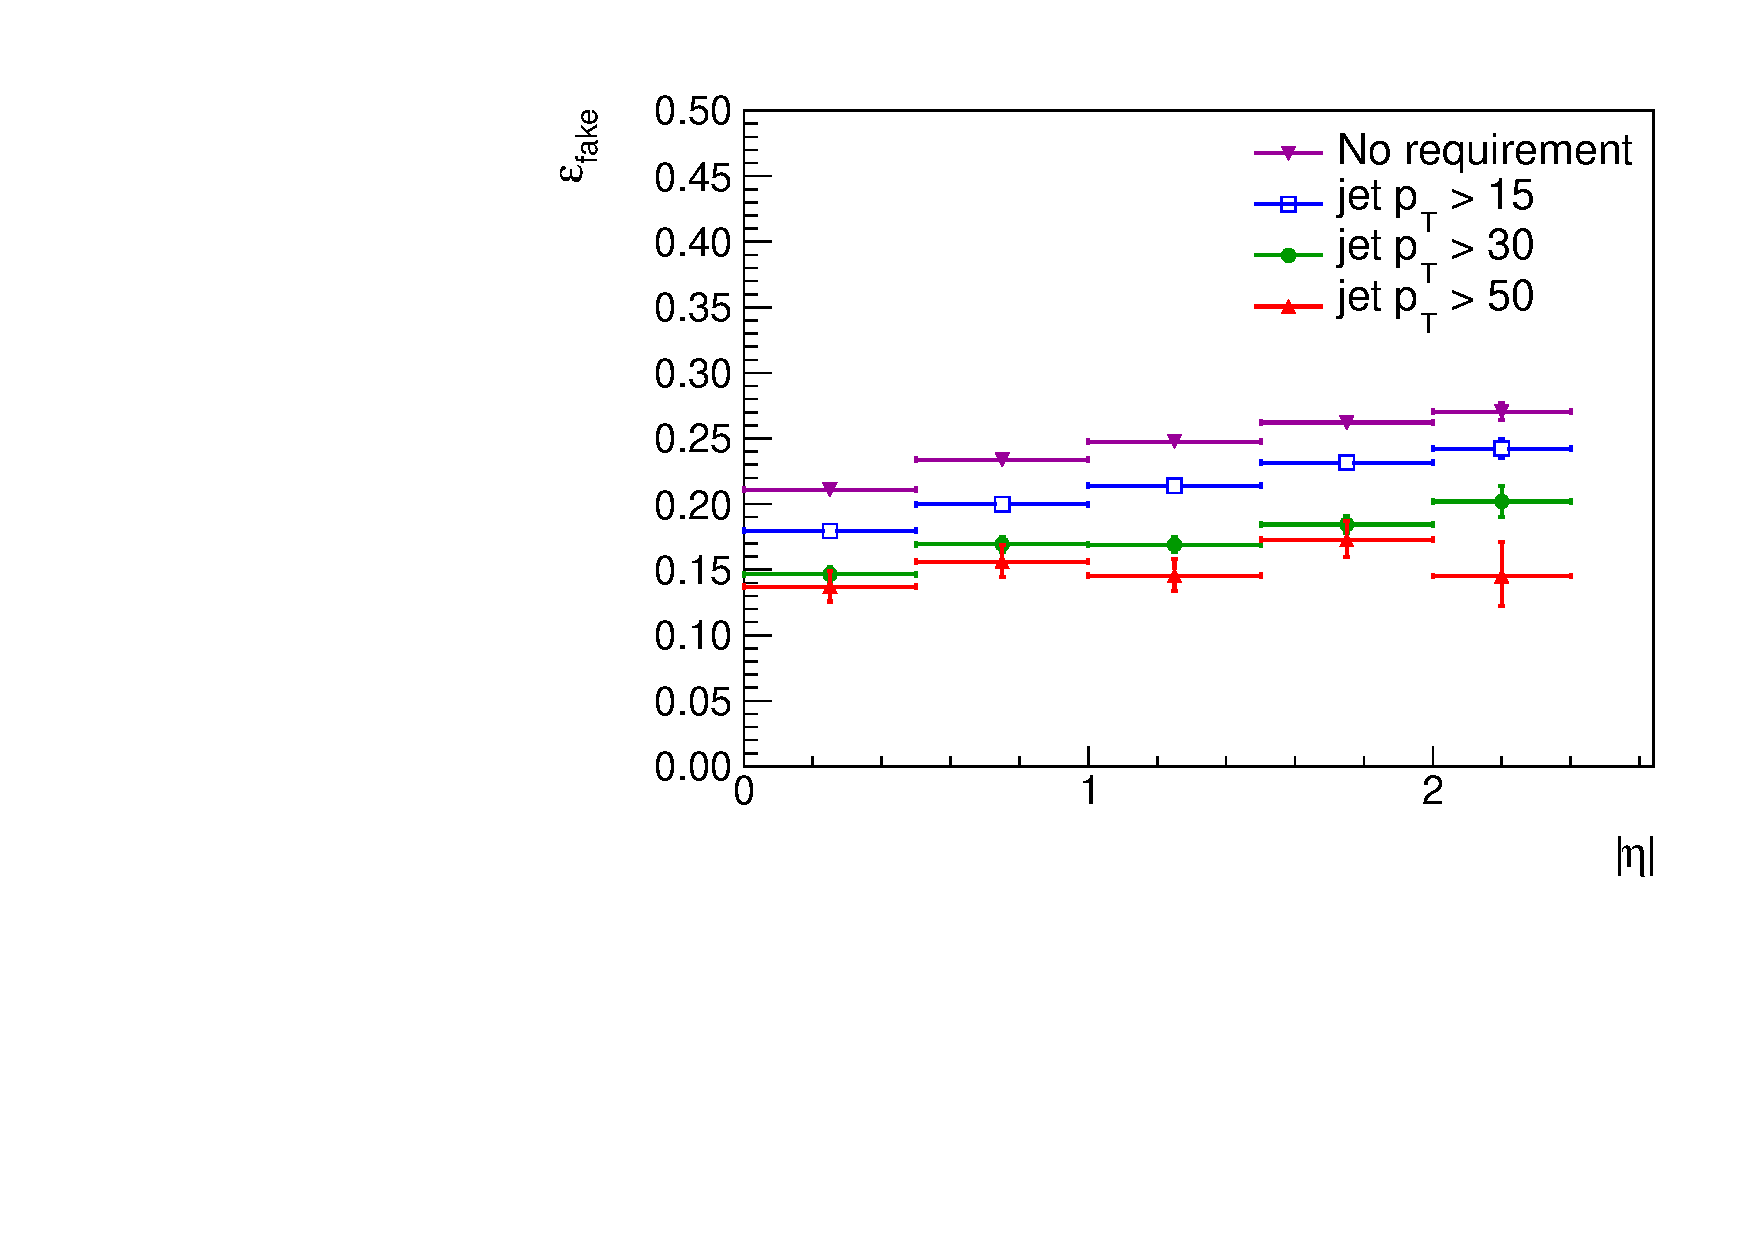
\includegraphics[width=0.45\textwidth]{figures/muon_freta_jetscan_m2.pdf}
\caption{Fake rates for M2 projected onto $p_T$ and $\eta$.}
\label{fig:mu_fr_iso04}

\end{center}
\end{figure}
